\documentclass{article}
\usepackage{amsfonts}
\usepackage[utf8]{inputenc}
\usepackage[T1]{fontenc}
\usepackage{float}
\usepackage{bbm}
\usepackage[round]{natbib}
\usepackage{hyperref}
\usepackage{graphicx} % Required for inserting images
\usepackage{tikz}
\usepackage{parskip} % Add this to remove paragraph indentation
\usetikzlibrary{shapes,arrows,positioning,fit}
\usepackage{listings}
\usepackage{amsthm}  % Add this package for theorem-like environments
\usepackage{xcolor}
\usepackage{amsmath}
\usepackage{mathabx}
\usepackage{subcaption}  % For subfigures
\usepackage{algorithmicx}
\usepackage{algpseudocode}
\usepackage{enumitem} % Added for better enumeration control
\bibliographystyle{plain}

% Define theorem-like environments
\theoremstyle{definition}
\newtheorem{definition}{Definition}
\newtheorem{remark}{Remark}

% Path to the images
\graphicspath{{./markdown_ugeopgave/Ugeopgave_3/}}

\title{Algoritmer og Datastrukturer (NDAA04010U) Ugeopgave 3}
\author{Københavns Universitet}
\date{2025}

\begin{document}

\maketitle

\section{Parallelle algoritmer}

I denne opgave er vi interesseret i at tælle trekanter i en simpel, uorienteret graf $G = (V, E)$, dvs. tripler af knuder $u, v, w \in V$ hvor alle par af knuder er kanter, dvs. $\{u, v\} \subseteq E$, $\{u, w\} \subseteq E$, $\{v, w\} \subseteq E$. Lad $v_1, \ldots, v_n$ være en nummerering af de $n$ knuder i $V$. Incidensmatricen $M(E)$ er en symmetrisk $n$-gange-$n$ matrix hvor $M(E)_{ij} = 1$ hvis $\{v_i, v_j\} \in E$ og $M(E)_{ij} = 0$ hvis $\{v_i, v_j\} \notin E$. Antag at $n$ er en potens af 2.

\begin{enumerate}[label=\alph*)]
\item Argumentér for at matricen $P = M(E)^2$ har egenskaben at $P_{ij}$ er lig med antal stier af længde præcis 2 der forbinder $v_i$ og $v_j$.

Lad $M(E)_{i*}$ være række $i$ i incidensmatricen, og $M(E)_{*j}$ være kolonne $j$. Ved matrixmultiplikation får vi:
$$P_{ij} = M(E)^2_{ij} = \sum_{k=1}^{n} M(E)_{ik} \cdot M(E)_{kj}$$

Hvert led i summen er produktet $M(E)_{ik} \cdot M(E)_{kj}$, som er 1 hvis og kun hvis både $\{v_i, v_k\} \in E$ og $\{v_k, v_j\} \in E$, dvs. hvis der findes en sti af længde 2 fra $v_i$ til $v_j$ via $v_k$. Summen tæller derfor præcis antallet af knuder $v_k$, der forbinder $v_i$ og $v_j$ med en sti af længde 2.

\item Brug resultatet fra a) til at designe en parallel algoritme der tæller antal trekanter i en graf. Du kan antage at input til algoritmen er en incidensmatrix $M(E)$.

En trekant i grafen består af tre knuder $v_i$, $v_j$ og $v_k$, hvor alle par er forbundet med kanter. For at tælle trekanter kan vi udnytte, at hvis $\{v_i, v_j\} \in E$ og $P_{ij}$ angiver antal stier af længde 2 mellem $v_i$ og $v_j$, så bidrager hver trekant der indeholder både $v_i$ og $v_j$ med én sti af længde 2.

\textbf{Algoritme:}
\begin{enumerate}
\item Beregn $P = M(E)^2$ parallelt ved hjælp af en effektiv parallel matrixmultiplikationsalgoritme.
\item Beregn $T = M(E) \circ P$, hvor $\circ$ er Hadamard-produkt.
\item Summen $\sum_{i,j} T_{ij}$ tæller hver trekant præcis 6 gange (én gang for hver permutation af de tre knuder) gøres parallel med( Gather + Reduce ).
\item Returner $\frac{1}{6}\sum_{i,j} T_{ij}$ som det endelige resultat.
\end{enumerate}

Når vi beregner $P = M(E)^2$, får vi at $P_{ab}$ er antallet af knuder $v_k$ sådan at både $\{v_a, v_k\}$ og $\{v_k, v_b\}$ er kanter. For at identificere en trekant med knuder $v_a$, $v_b$ og en tredje knude $v_k$, skal vi kontrollere:
\begin{itemize}
\item $\{v_a, v_k\} \in E$ og $\{v_k, v_b\} \in E$ (dette tælles af $P_{ab}$)
\item $\{v_a, v_b\} \in E$ (dette angives af $M(E)_{ab}$)
\end{itemize}

Ved at beregne $T = M(E) \circ P$ får vi:
\begin{itemize}
\item $T_{ab} = M(E)_{ab} \cdot P_{ab}$
\item $T_{ab} > 0$ hvis og kun hvis der er både en direkte kant mellem $v_a$ og $v_b$ OG mindst én sti af længde 2 mellem dem
\item $T_{ab}$ angiver præcis antallet af trekanter der indeholder kanten $\{v_a, v_b\}$
\end{itemize}

\item Hvad er span og arbejde for din algoritme fra b) hvis du gør brug af en algoritme til matrixmultiplikation der har arbejde $T_1$ og span $T_\infty$? Giv svar som funktion af $n$, $T_1$, $T_\infty$.

Vi har følgende operationer med span og arbejde:

\begin{enumerate}
    \item Matrixmultiplikation: arbejde=$T_1$ span=$T_\infty$
    \item Hadamard-produkt: arbejde=$n^2$ span=1
    \item Gather: arbejde=$n^2$ span=1
    \item Reduce(addition): arbejde=$n^2$ span=$\log(n^2)=2\log(n)$
\end{enumerate}

Dvs. 
\[
\text{total arbejde} = T_1 + 3n^2
\]

\[
\text{total span} = T_\infty + 1 + 1 + 2\log(n) = T_\infty + 2 + 2\log(n)
\]

\end{enumerate}

\section{Amortiseret analyse}

I denne opgave betragter vi potentialfunktionen der bruges til at analysere dynamiske tabeller i CLRS sektion 16.4.1. Lad $\Phi_i$ betegne potentialfunktionens værdi efter $i$ Table-Insert operationer, uden nogen Table-Delete operationer. Hvilke egenskaber har $\Phi_i$? Vælg ét eller flere korrekte svar og beskriv hvordan du kom frem til dem (både positive og negative svar).

\begin{enumerate}
\item $\Phi_i = \Omega(1)$.
\item $\Phi_i = O(1)$.
\item $\Phi_i = \Omega(i)$.
\item $\Phi_i = O(i)$.
\item $\Phi_i \geq \Phi_{i-1}$.
\item $\Phi_i \geq 0$.
\end{enumerate}

\section{Rød-sorte søgetræer}

Betragt et rød-sort binært søgetræ $T$ (eng. red-black binary search tree), som beskrevet i CLRS kapitel 13. Betragt nedenstående træ, hvor alle blade er udeladt (som på CLRS figur 13.1.c) og to indre knuder er uspecificerede:

\begin{figure}[H]
    \centering
    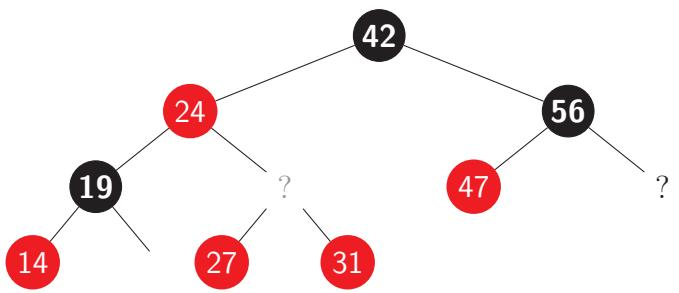
\includegraphics[width=0.7\textwidth]{_page_1_Figure_5.jpeg}
    \caption{Rød-sort binært søgetræ med uspecificerede knuder}
\end{figure}

Hvilke knuder er mulige på mindst én af positionerne markeret med ?, hvis træet skal overholde invarianterne for et rød-sort binært søgetræ? Vælg ét eller flere korrekte svar og beskriv hvordan du kom frem til dem (både positive og negative svar).

\begin{enumerate}
\item En rød knude med nøglen 28.
\item En rød knude med nøglen 44.
\item En rød knude med nøglen 58.
\item En sort knude med nøglen 25.
\item En sort knude med nøglen 30.
\item En sort knude med nøglen 66.
\end{enumerate}

\section{Indsættelse i rød-sorte søgetræer}

Betragt dette rød-sorte binære søgetræ (eng. red-black binary search tree), hvor bladene er udeladt på tegningen:

\begin{figure}[H]
    \centering
    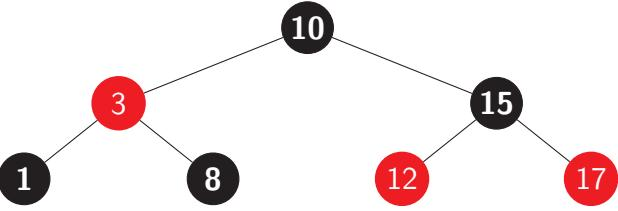
\includegraphics[width=0.7\textwidth]{_page_2_Figure_0.jpeg}
    \caption{Rød-sort binært søgetræ}
\end{figure}

Antag at vi bruger indsættelsesalgoritmen RB-Insert fra CLRS kapitel 13 til at indsætte nøglen 9. Hvad sker med træet? Vælg præcis ét svar og beskriv hvordan du kom frem til det.

\begin{enumerate}
\item 9 indsættes som højre barn til knude 8 og farves rød.
\item 9 indsættes som højre barn til knude 8 og farves sort.
\item 9 indsættes som venstre barn til knude 12 og farves rød.
\item 9 indsættes som venstre barn til knude 12 og farves sort.
\item Ingen af ovenstående.
\end{enumerate}

\section{Køretid for rød-sorte søgetræer}

Betragt et rød-sort binært søgetræ $T$ (eng. red-black binary search tree), som beskrevet i CLRS kapitel 13, hvorpå der (startende med et tomt træ) udføres $n_1$ Insert operationer, $n_2$ Delete operationer, og $n_3$ Search operationer (sidstnævnte kaldes også "access" operationer). Det totale antal operationer er $N = n_1 + n_2 + n_3$. Hvilke af følgende udsagn er altid sande? Vælg ét eller flere korrekte svar og beskriv hvordan du kom frem til dem (både positive og negative svar).

\begin{enumerate}
\item Den samlede tid for operationerne er $\Omega(N)$.
\item Den samlede tid for operationerne er $O(N \lg N)$.
\item Den samlede tid for operationerne er $O(n_3 + (n_1 + n_2) \lg N)$.
\item Dybden af $T$ er højst $2 \lg(n_1 + 1)$.
\item Alle blade i $T$ er i dybde mindst $\lfloor\lg(n_3 + 1)\rfloor$.
\item Alle sorte knuder i $T$ har en afstand til roden, der er et lige tal.
\end{enumerate}

\end{document}


\bibliographystyle{plainnat}
\bibliography{references}